\documentclass[10pt]{article}

\usepackage[hmargin=20mm, vmargin=12mm]{geometry}
\usepackage{lmodern}
\usepackage{parskip}
\usepackage{amsmath}
\usepackage{graphicx}
\usepackage{animate}
\usepackage[nodisplayskipstretch]{setspace}
\usepackage{titling}
\usepackage{sectsty}
\usepackage{changepage}
\usepackage{float}
\setstretch{0.5}
\setlength{\abovedisplayskip}{0pt}
\setlength{\belowdisplayskip}{0pt}
\graphicspath{ {../figures/} }

\pretitle{\begin{center}\fontsize{12bp}{12bp}\selectfont}
\posttitle{\end{center}}
\preauthor{\begin{center}\fontsize{10bp}{10bp}\selectfont}
\postauthor{\end{center}}
\predate{}
\date{}
\postdate{}

\sectionfont{\fontsize{11bp}{11bp}\selectfont}
\subsectionfont{\fontsize{10bp}{10bp}\selectfont}
\begin{document}
\title{Data, Estimation and Inference Report}
\author{Ben Ellis}
\maketitle
% Describe the data that we are trying to fit and its patterns
This report considers data from a sensor measuring tide height.
The sensor often fails to transmit readings due to severe weather, and 
hence we here try to interpolate from the data available.

The readings from the sensor and the true tide heights over the period 
considered are shown in Figure~\ref{fig:scatter} in the Appendix. 


This data exhibits a few interesting patterns:
\begin{itemize}
    \item As we would expect, the tide height is periodic with a period of roughly 12 hours.
    \item There are a few notable sections where data are entirely missing.
    \item Although data are missing, observed readings show little, and uniform, noise. 
\end{itemize}

The regular structure of the data suggests that we could use Gaussian Processes to interpolate.

\section*{Gaussian Processes}

A Gaussian process $f(\mathbf{x}) \sim \mathcal{GP}(m(\mathbf{x}), K(\mathbf{x}, \mathbf{x}))$ is a collection
of random variables, any finite collection of which is Gaussian distributed. 
%More specifically, any finite collection 
%of function values $f(\mathbf{x}_1), \dots, f(\mathbf{x}_n)$ will have the distribution
% \[
%     \begin{bmatrix}
%         f(\mathbf{x}_1) \\
%         f(\mathbf{x}_2) \\
%         \vdots \\
%         f(\mathbf{x}_n)
%     \end{bmatrix} \sim 
%     \mathcal{N}\begin{pmatrix}
%         \begin{bmatrix}
%             m(\mathbf{x}_1) \\
%             m(\mathbf{x}_2) \\
%             \vdots \\
%             m(\mathbf{x}_n)
%         \end{bmatrix}, 
%         \begin{bmatrix}
%             K(\mathbf{x}_1, \mathbf{x}_1) & K(\mathbf{x}_1, \mathbf{x}_2) & \dots & K(\mathbf{x}_1, \mathbf{x}_n) \\
%             K(\mathbf{x}_2, \mathbf{x}_1) & K(\mathbf{x}_2, \mathbf{x}_2) & \dots & K(\mathbf{x}_2, \mathbf{x}_n) \\
%             \vdots & \vdots & \ddots & \vdots \\
%             K(\mathbf{x}_n, \mathbf{x}_1) & K(\mathbf{x}_n, \mathbf{x}_2) & \dots & K(\mathbf{x}_n, \mathbf{x}_n)
%         \end{bmatrix}
%     \end{pmatrix}
% \]
$m$ is a function which gives the value of the mean of the Gaussian at its input, and $K$ is a kernel function which given
inputs $\mathbf{x}_i$ and $\mathbf{x}_j$ computes the entry in the covariance matrix $\Sigma_{ij}$. Hence for any point
$\mathbf{x}_{\star}$ the Gaussian process induces a Gaussian distribution of the possible function values $f(\mathbf{x}_{\star})$.
This is shown for a simple linear case in Figure~\ref{fig:func_distribution} in the Appendix. More than that though, the Gaussian process also gives
a joint Gaussian distribution for any discrete set of points $X_{\star}$, meaning that this allows us to control the variation in the
function between points by specifying the kernel function. 
\subsection*{Inference in Gaussian Processes}
To perform inference, we must use the Gaussian Process (GP) to predict the function values $\mathbf{f}_{\star}$ at some set of points
$X_{\star}$ given noisy observations $\mathbf{y}$ at a set of points $X$. We assume that a single observation $y_i$ is affected by
IID Gaussian noise and hence the observations $\mathbf{y}$ and function values $\mathbf{f}_{\star}$ are jointly Gaussian.
% \begin{align*}
%     y_i &= f(\mathbf{x}_i) + \epsilon_i \\
%     \epsilon_i &\sim \mathcal{N}(0, \sigma^2)
% \end{align*}
% The observations $\mathbf{y}$ and function values $\mathbf{f}_{\star}$ that we wish to predict are jointly Gaussian. This is because the 
% covariance matrix of $\mathbf{y}$ is
% \[
%     \text{cov}(\mathbf{y}) = K(X, X) + \sigma^2 I
% \]
\[
    \begin{bmatrix}
        \mathbf{y} \\
        \mathbf{f}_{\star}
    \end{bmatrix} \sim
    \mathcal{N}\begin{pmatrix}
        \mathbf{0}, & 
        \begin{bmatrix}
            K(X, X) + \sigma^2 I & K(X, X_{\star}) \\
            K(X_{\star}, X) & K(X_{\star}, X_{\star}) 
        \end{bmatrix}
    \end{pmatrix}
\]
where we have assumed that the mean is $\mathbf{0}$. In this case we normalised the data to zero mean and unit variance to achieve this.
The identity matrix is used here because of the IID assumption about our noise.
Since the conditionals of a Gaussian are also Gaussian, this gives us the posterior distribution
\begin{align*}
p(\mathbf{f}_{\star} \left| \mathbf{y}, X, X_{\star}\right.) &= \mathcal{N}(\mathbf{m}_{\star}, \mathbf{K}_{\star}) \\
\mathbf{m}_{\star} &= K(X_{\star}, X) (K(X, X) + \sigma^2 I)^{-1} \mathbf{y} \\
\mathbf{K}_{\star} &= K(X_{\star}, X_{\star}) - K(X_{\star}, X) (K(X, X) + \sigma^2 I)^{-1} K(X, X_{\star})
\end{align*}
\subsection*{Choice of Kernel Function}
The expression for the posterior above shows that when the observed data has low covariance with the data we wish to predict 
(i.e.\ when $K(X_{\star}, X)$ is filled with small values compared to $K(X_{\star}, X_{\star})$), the posterior will
revert to the prior distribution specified by the GP\@. It is therefore important to correctly formulate the kernel function and mean
depending on the data. For the mean, we assumed a constant mean of 0 after normalising the data. Choosing a kernel function must be done
with some more care. The tide data is periodic, however there is also some variation
in the height of the peaks and troughs. Therefore in this report the kernel function used is a combination of the periodic and RBF kernels, as below.

\begin{align*}
    K(x, x') &= K_{\text{periodic}}(x, x') + \alpha K_{\text{rbf}}(x, x') \\
    K_{\text{periodic}}(x, x') &= \sigma_p^2 \exp\left(- \frac{2\left(\sin(\pi d(x, x') / p)\right)}{\omega_p}\right) \\
    K_{\text{rbf}}(x, x') &= \sigma_r^2 \exp\left(- \frac{\|x - x'\|^2}{2\omega_r}\right)
\end{align*}

where $d(x, x')$ is the euclidean distance between two points $x$ and $x'$. I found this combination made it easier to fit both the variation
in height of the peaks and the periods of the function because it allows periodic and adjacent similarity to be balanced. 
This kernel function
has a number of hyperparameters, which we must optimise over.
% which control the period ($p$), the uncertainty away from data ($\sigma_p$ and $\sigma_r$), and the scale
% over which the function varies ($\omega_r$ and $\omega_p$). We will collect all of these together with $\alpha$ and refer to them by 
%$\mathbf{\phi}$. 
We do not optimise over the noise variance $\sigma$, but it was estimated to 1 significant figure from the data as $0.03$. 

\subsection*{Optimising Hyperparameters}

To choose the hyperparameters, we do some optimisation. The quantity that we optimise is the marginal likelihood:
\begin{align*}
    p(\mathbf{y} | X) &= \int p(\mathbf{y} | \mathbf{f}, X) p(\mathbf{f} | X) \text{d}\mathbf{f} \\
                      &= \mathcal{N}(\mathbf{0}, K(X, X) + \sigma^2 I)
\end{align*}
This quantity measures, for a particular set of hyperparameters, the probability density of the observations that we recorded across all 
possible function draws. This is different to the likelihood $p(\mathbf{y} | \mathbf{f}, X)$, which only considers one particular function
drawn from the distribution. I optimised the log-marginal likelihood with the standard SciPy implementation of LBFGS-B.

\section*{Experiments}

I first fit a Gaussian Process with the kernel specified above to the whole dataset. This is shown in Figure~\ref{fig:gp}. 
This was obtained by specifying an initial guess for the hyperparameters chosen by hand, and the optimising them as above. The prediction of
the mean on this data is clearly very well fit, but the uncertainty prediction could be better. Its form is good because the uncertainty is
greater when there is a poverty of data, and low when nearby sensor data is available. Moreover, the uncertainty is higher when predicting the
peaks and troughs than the data in between, which appears more regular. However, the overall uncertainty is unreasonably low, particularly in
larger regions where there is little or no data. 

\begin{figure}
\begin{minipage}{.5\textwidth}
    \centering
    \includegraphics[width=\textwidth]{rbf_and_periodic}
    \caption{Plot showing the fit of the Gaussian Process to the normalised tide height}\label{fig:gp}
\end{minipage}
\begin{minipage}{.5\textwidth}
    \centering
    \animategraphics[loop,autoplay, controls=all, width=\textwidth]{0.25}{animation/sequential_prediction-}{0}{9}
    \caption{Animation showing randomly initialised models fitted to progressively larger portions of the dataset.
            This will animate when opened with Adobe Acrobat Reader.}\label{fig:seq_prediction}
\end{minipage}
\end{figure}
\subsection*{Sequential Prediction}

To explore the uncertainty estimates further, I looked at sequential predictions on the sensor data. The results are shown in the animation
in Figure~\ref{fig:seq_prediction}. This can be viewed in Adobe Acrobat. In this task I split the data into 10 chunks, and then fit a GP starting
from random initial hyperparameters using the method above on progressively larger numbers of chunks. With the bounds I was using
for the whole data set, random initialisations had very variable performance. I therefore used much tighter bounds with the random initial 
seeds to allow the GP to fit the data properly, while avoiding narrowing the search to a known set of good parameters. 

For the first 10\% of the data, the GP has not seen enough data to correctly estimate the period. It therefore guesses slightly incorrectly 
and is far too certain about the data in some sections. The model fit on 20\% of the data is similar, although its
uncertainty is much higher. In both cases there is likely not enough data for the GP to understand how uncertain it should be. If the
model has not seen at least 1 period, it cannot possibly estimate the period, or the variation in the data across periods. The third model
has correctly fit the period, but not correct uncertainty estimates. I think this is caused in part by there being little
variation in the heights of the first three periods compared with the fourth, which is much lower. The fourth model does better, and the 
fifth is the first that truly fits the rest of the data reasonably, with none of the periods representing significant deviations from its
expectations.
After this, the differences between the models are largely due to random variation. The eigth model is particularly poor, which I
believe is due to poor optimisation performance. The model before it had a maximum marginal likelihood of 1154, compared to its value of 1054.
I would expect this to usually increase with more data. 

% Why use gaussian process here? 
% Looks like a fairly regular function so limited expressivity not a problem
% Describe gaussian processes 
% Describe the marginal likelihood.
% Talk about 0 mean assumption and normalisation of data
% Talk about kernel choice. 
\appendix
\section{Supplementary Figures}


\begin{figure}[H]
\centering
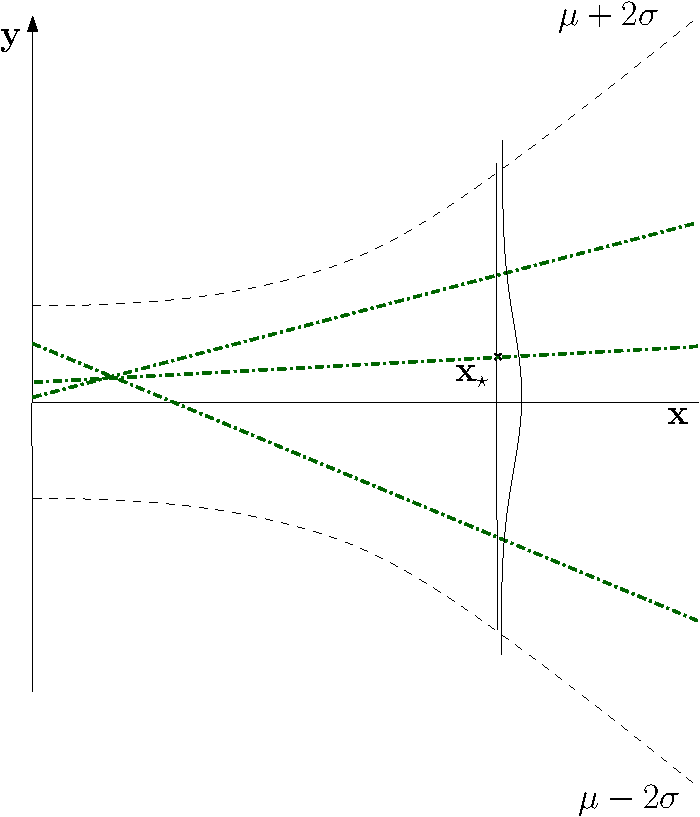
\includegraphics[width=0.4\linewidth]{function_distribution_cropped}
\caption{Diagram illustrating a Gaussian distribution over function values at $\mathbf{x}_{\star}$. Some simple functions drawn
from the distribution are shown in dark green.}\label{fig:func_distribution}
\end{figure}
\begin{figure}[H]
    \centering
    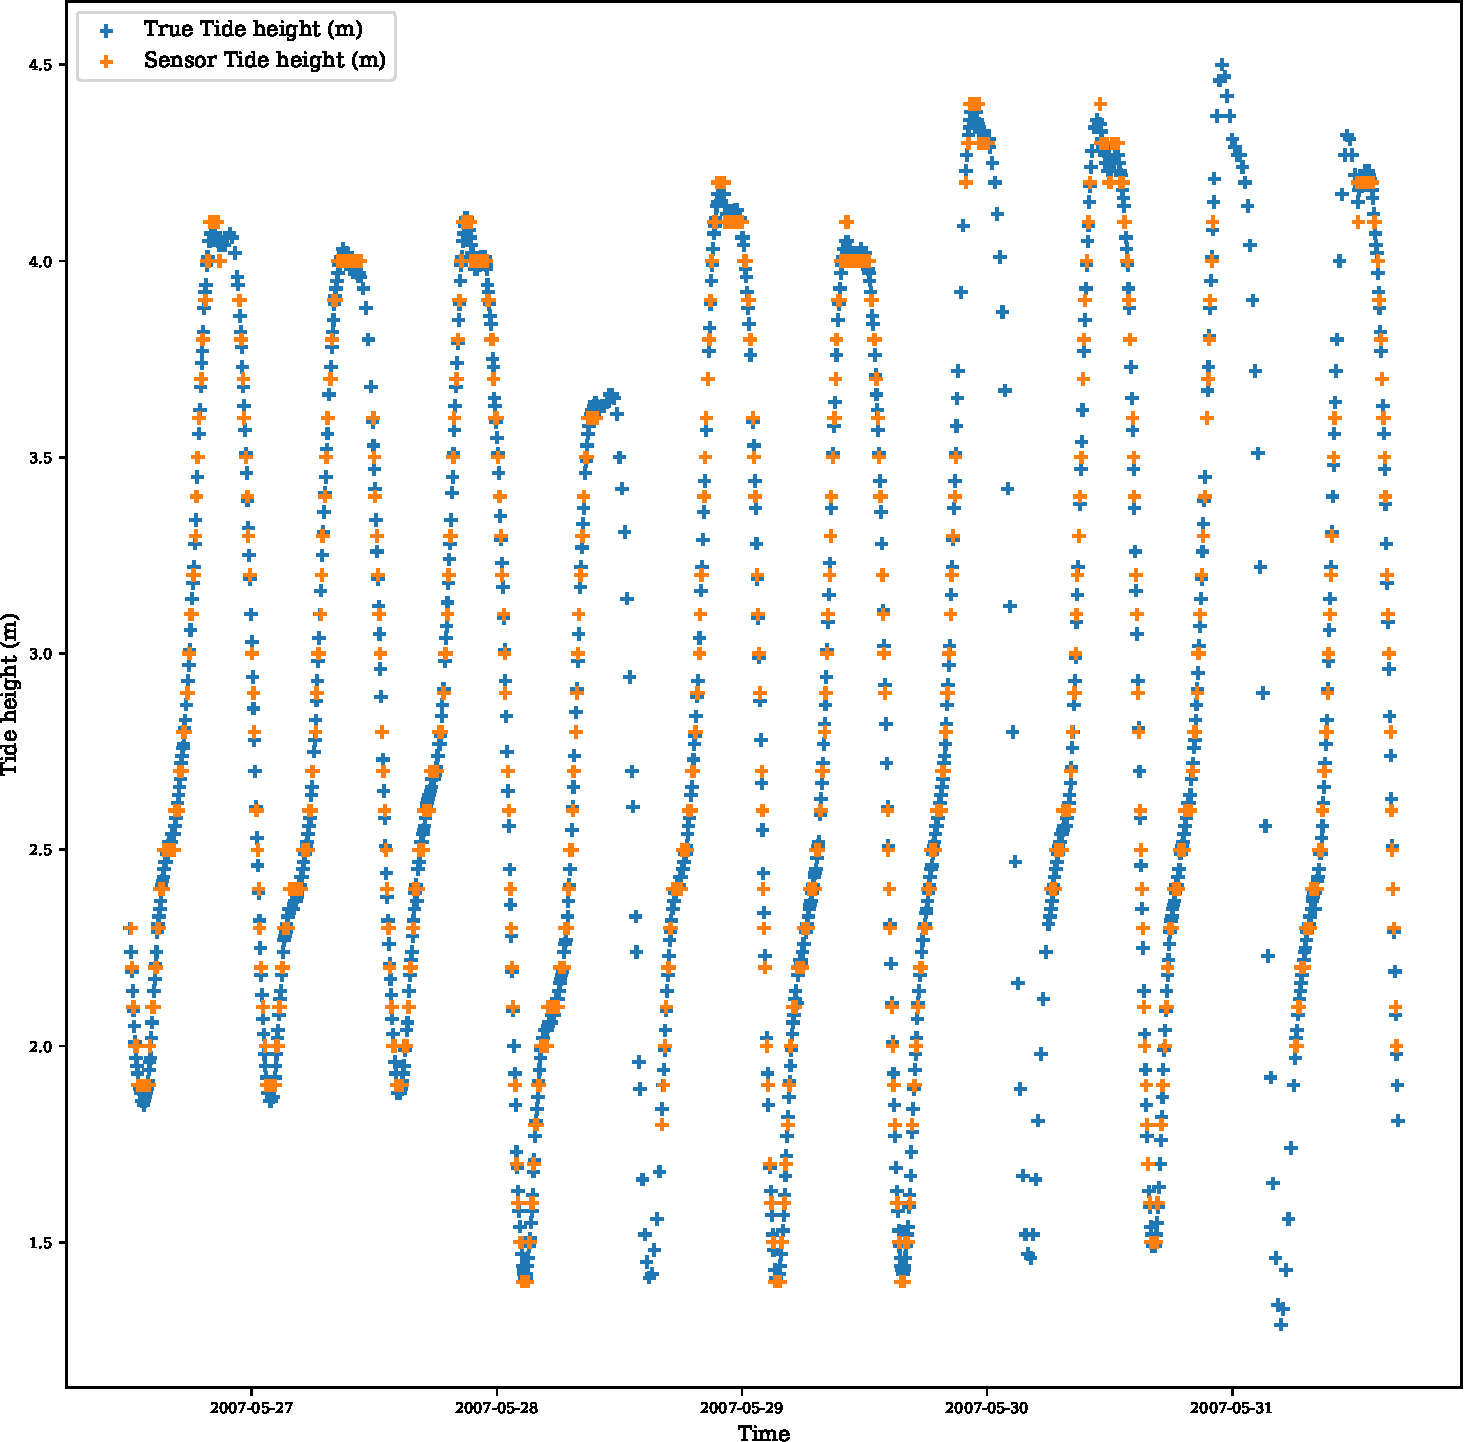
\includegraphics[width=0.5\linewidth]{sensor_scatter_cropped}
    \caption{Scatter plot of the data obtained by the sensor and the true tide height}\label{fig:scatter}
\end{figure}




\end{document}

